\section{Transport Layer Security \& Encryption}
Before, all communication sent ``\textbf{over the wire}'' (from device to device),
was sent ``\textbf{in the clear}'' (unencrypted). This means that anyone could 
view data sent between devices in plain text. This is a problem when setting up 
infrastructure such as banking, e-commerce, or any other service that requires
sensitive information to be sent over the internet.

\begin{Def}[Integrity \& Authenticity]

    \textbf{Integrity} is the assurance that data has not been altered in transit.\\
    \textbf{Authenticity} is the assurance that the data is coming from the correct source.
\end{Def}
\begin{Def}[Transport Layer Security (TLS)]

    TLS is a protocol providing end-to-end encryption of data. It authenticates
    the server via \textbf{TLS certificates} to ensure the client is connecting to 
    the correct host. It also ensures integrity of the data.

    The Engineering Task Force (IETF) published the first version of TLS in 1999. As of 
    today the most recent version is TLS 1.3. (2018).
    \hfill \cite{cloudflare_tls}
\end{Def}

\begin{Def}[Secure Sockets Layer (SSL) [Deprecated]]

    SSL is the predecessor to TLS. It was developed by Netscape in the 1990s. 
    SSL 3.0 was released in 1996. SSL 3.0 was found to be insecure and was replaced
    by TLS 1.0 in 1999.
    \hfill \cite{cloudflare_tls}
\end{Def}

\begin{Def}[Certificate Authority (CA)]

    A CA is a third-party entity that issues digital certificates. Often called \textbf{SSL certificates} or TLS certificates.
    The protocol supports both SSL and TLS. Despite SSL's deprecation the name stuck due branding issues.
    Browsers and Operating systems have a list of trusted CAs called the \textbf{root store}.
    A full list of Microsoft's trusted CAs can be found here:\\ \href{https://ccadb.my.salesforce-sites.com/microsoft/IncludedCACertificateReportForMSFT}{https://ccadb.my.salesforce-sites.com/microsoft/...}
    \hfill \cite{kinsta_tls_ssl}
\end{Def}

\newpage 

\begin{Def}[Encryption]

    \textbf{Encryption} is the process of converting plaintext into ciphertext (indiscernible text).\\
    \textbf{Decryption} is the process of converting ciphertext back into plaintext.

\end{Def}
\begin{Def}[Symmetric \& Asymmetric Encryption]
    
    \textbf{Key}: is a seed/piece of information used to encrypt or decrypt data.\\
    \textbf{Symmetric Encryption}: uses the same key for both encryption and decryption.\\
    \textbf{Asymmetric Encryption}: uses a public key for encryption and a private key for decryption.\\
    ${}$ \hfill \cite{adetunji_symmetric_asymmetric_encryption}
\end{Def}

\vspace{-1em}
\begin{figure}[h!]
    \centering
    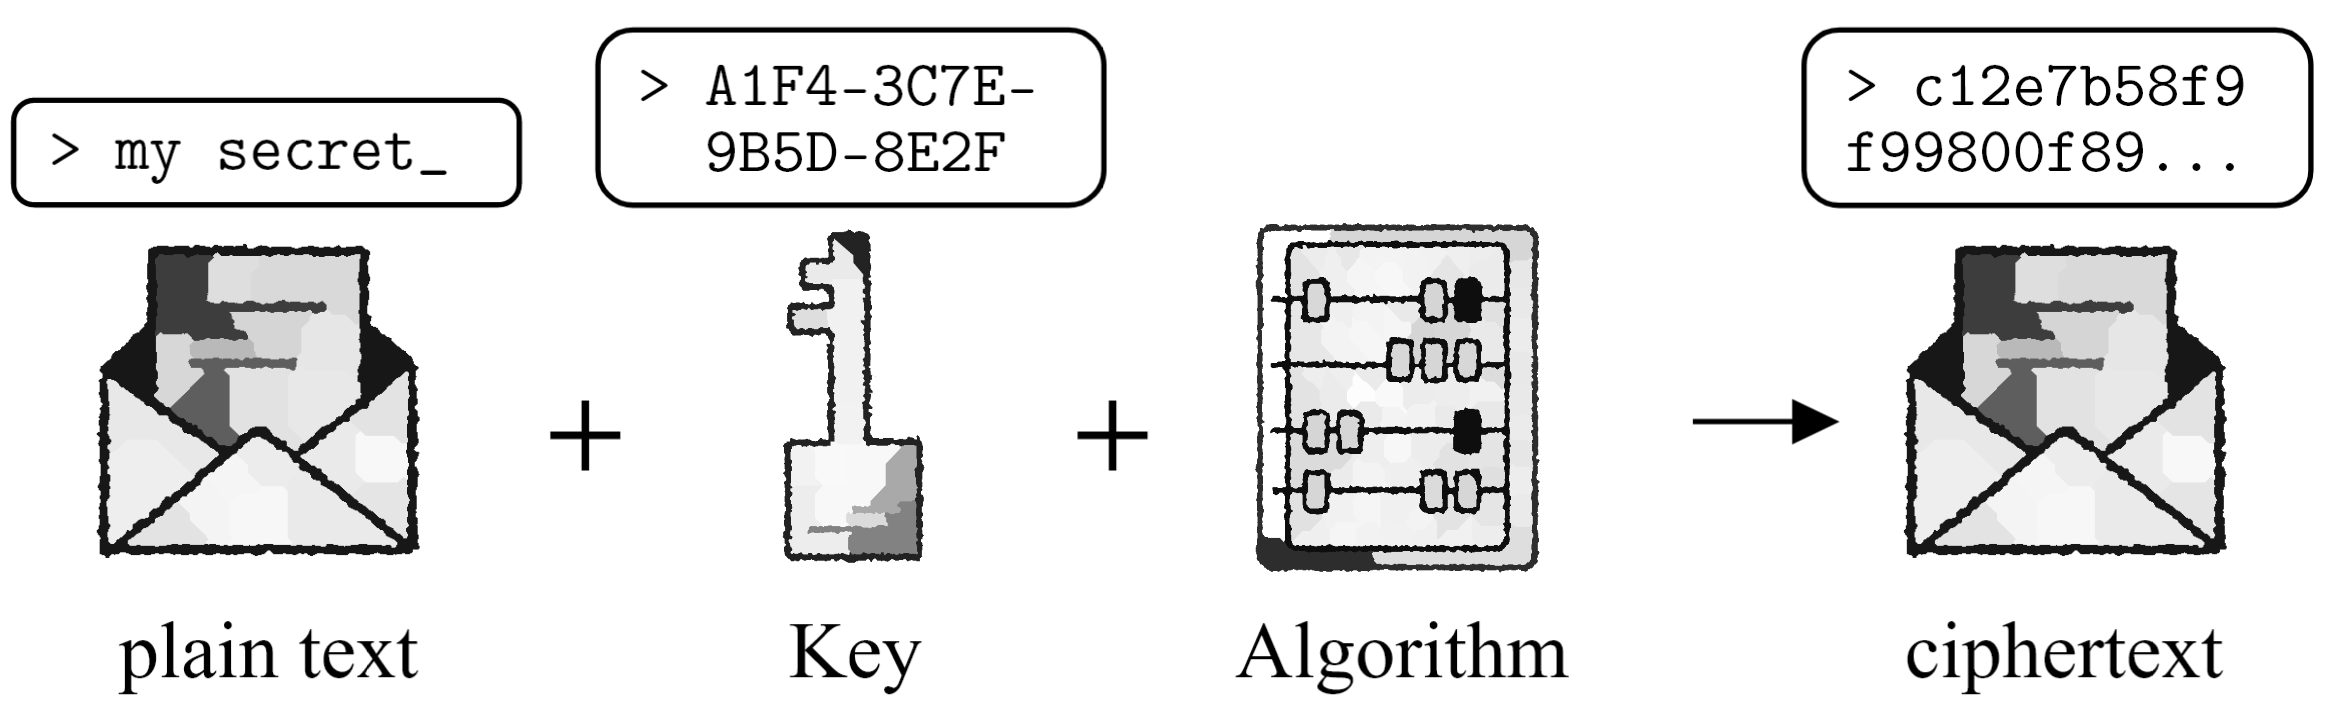
\includegraphics[width=1\textwidth]{Sections/sec/encrypt.png}
    \caption{High-level depiction of encryption.}
    \label{fig:encryption}
\end{figure}

\noindent
Encryption takes a key, data, and an algorithm to produce ciphertext.
Decryption takes the same key, ciphertext, and algorithm to produce the original data.

\vspace{1em}
\begin{Def}[Hashing]
    \textbf{Hashing} is the process of converting data into a fixed-length string of characters.
    Hashing is a one-way function, meaning it cannot be reversed (theoretically). In practice, 
    it is computationally infeasible to reverse a hash without brute force (trying all possible inputs) 
    or exploiting weaknesses in the hashing algorithm. Some hash algorithms use the text itself 
    as input, while others may incorporate a separate key (e.g., HMAC).
\end{Def}

\begin{Def}[Hypertext Transfer Protocol Secure (HTTPS)]

    A version of HTTP that uses TLS to encrypt data.
\end{Def}


\newpage 
\begin{Def}[SSL/TLS Certificate Specifications]

    \begin{itemize}
        \item \textbf{Common Name (CN)}: The domain name the certificate is issued for.
        \item \textbf{Subject Alternative Name (SAN)}: Additional domain names or subdomains covered by the certificate.
        \item \textbf{Key Length}: A minimum of 2048 bits, ensuring strong encryption.
        \item \textbf{Hashing Algorithm}: Typically SHA-256 for secure data integrity.
        \item \textbf{Valid From/To}: The validity period, usually up to 397 days.
        \item \textbf{Issuer}: The trusted Certificate Authority (CA) that issued the certificate.
        \item \textbf{Extended Key Usage}: Specifies purposes like server authentication or client authentication.
    \end{itemize}
    \hfill \cite{kinsta_tls_ssl}
\end{Def}

\begin{figure}[h!]
    \centering
    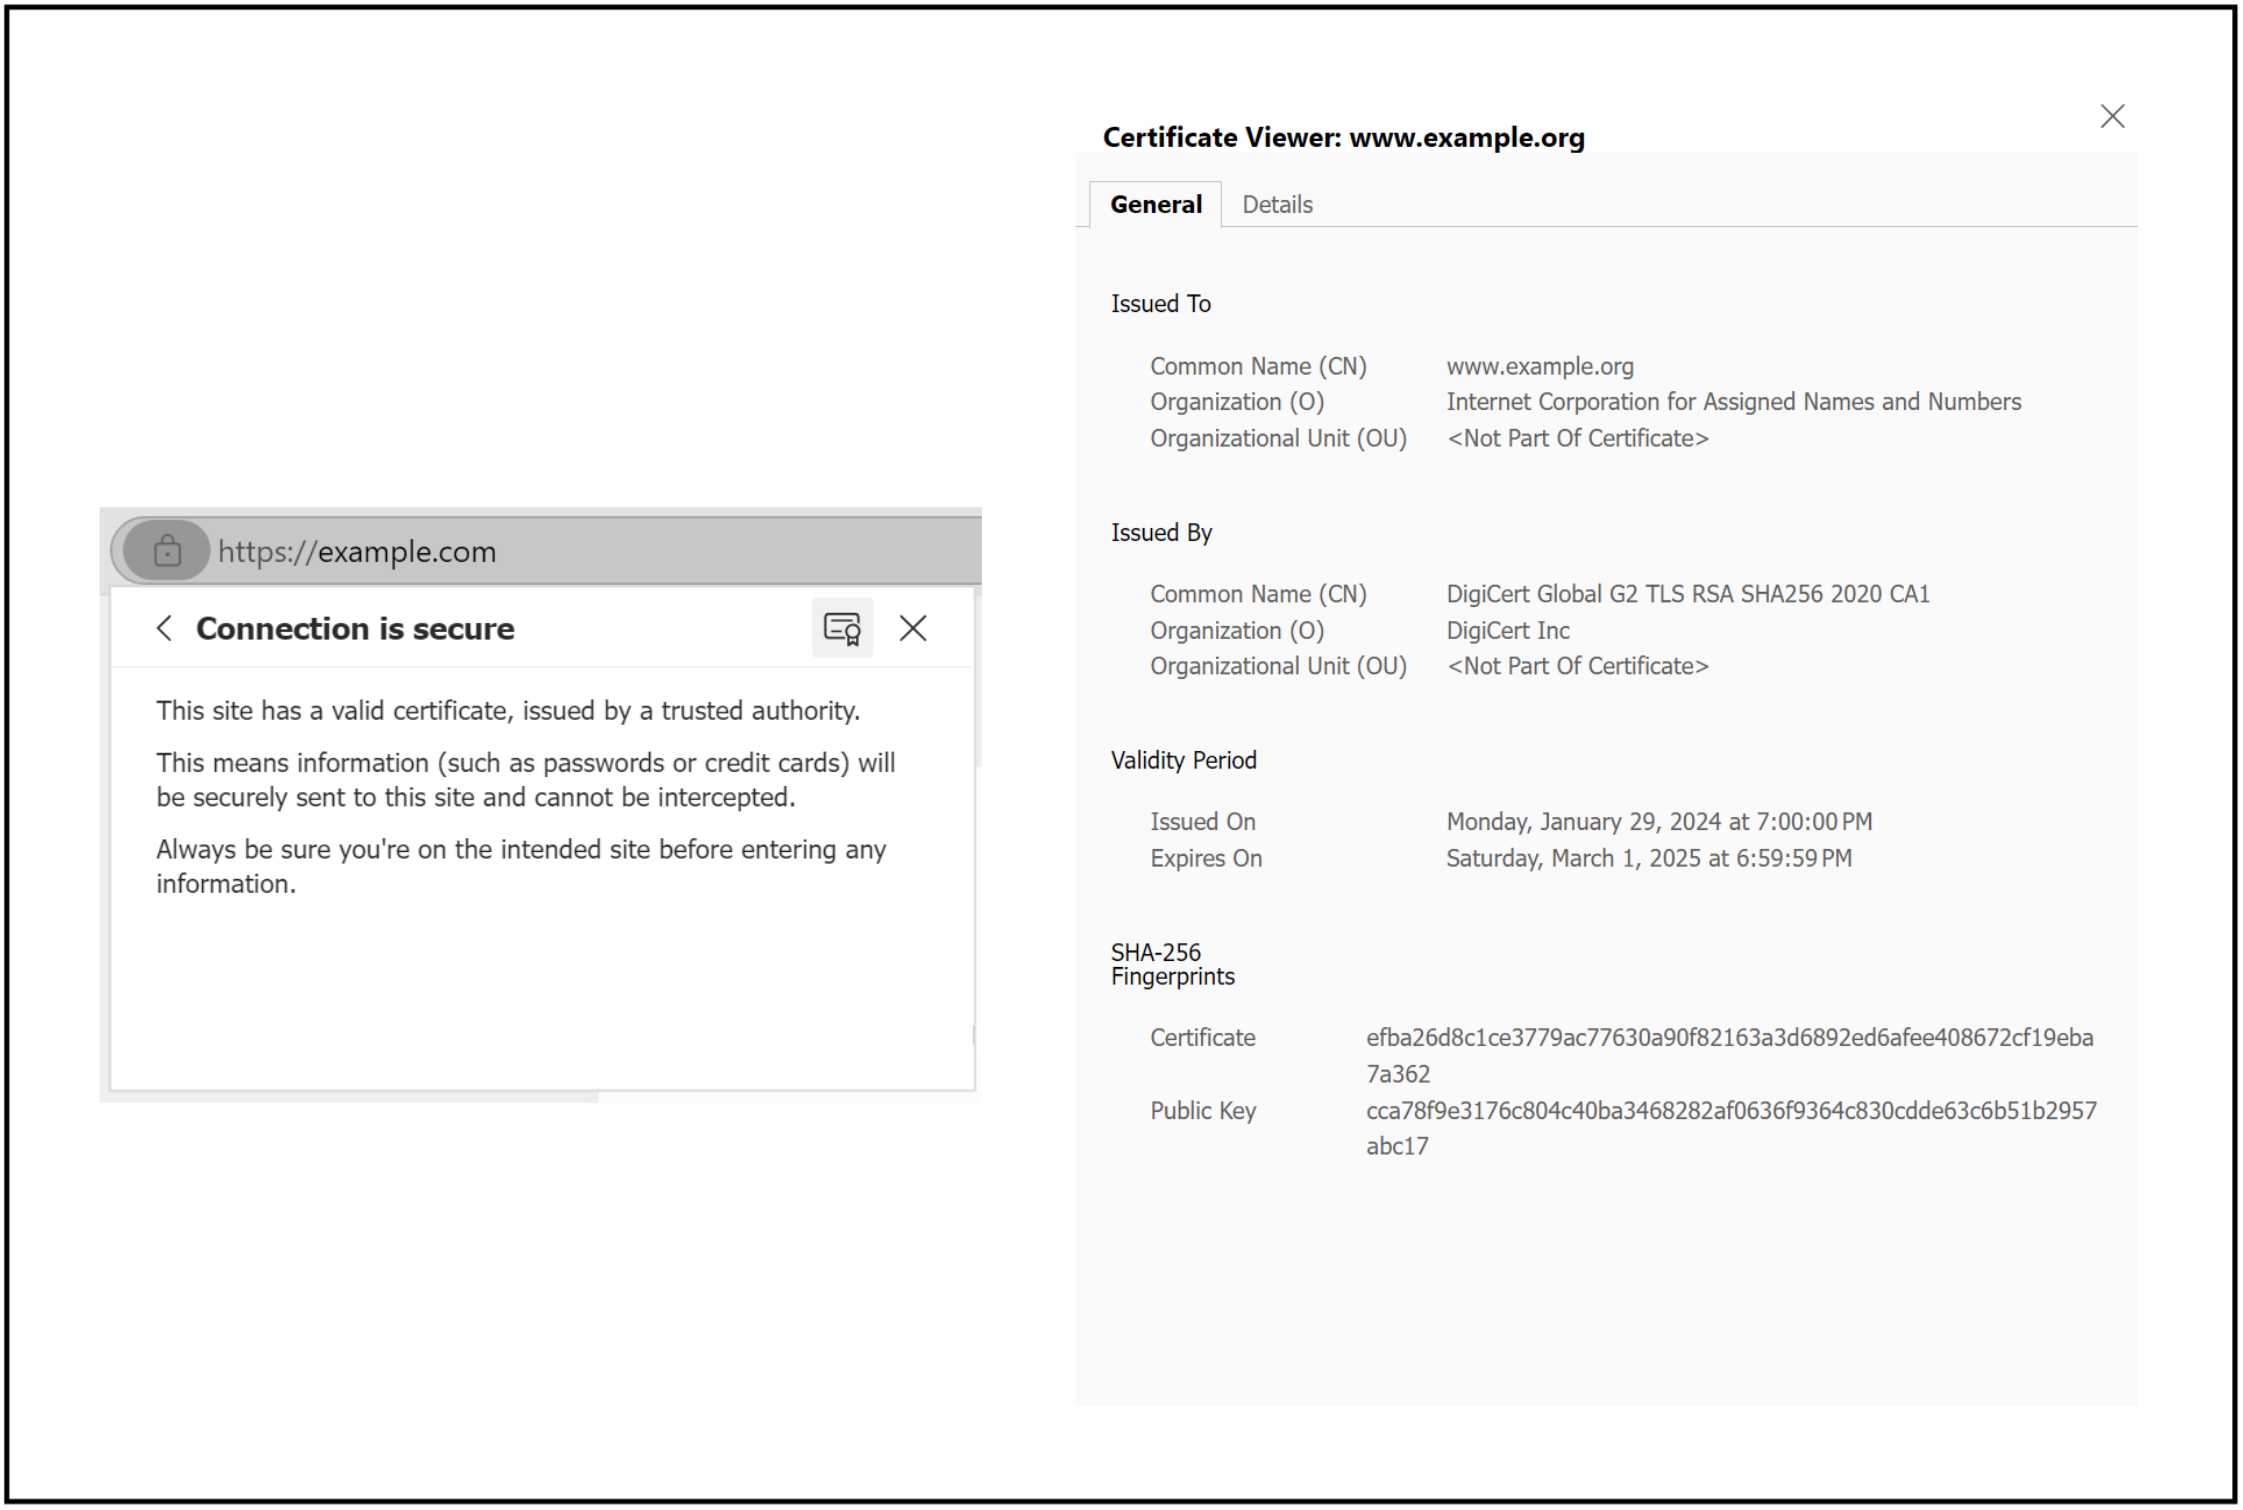
\includegraphics[width=1\textwidth]{Sections/sec/cert.png}
    \caption{SSL certificate obtained through the Edge browser on example.com}
    \label{fig:cert}
\end{figure}






